\section{Качественные задачи.}

\begin{enumerate}
\item Чем обусловлена способность теплового излучения находится в равновесии с
излучающими телами?

\item Объясните появление резкой границы излучения в области малых длин волн в
спектре тормозного рентгеновского излучения.

\item Чем обусловлено появление одновременно смещённой и несмещённой
компонент в спектре рассеяния рентгеновского излучения веществом (эффект
Комптона)?

\item Как зависит интенсивность смещённой и несмещённой компонент в спектре
рассеяния рентгеновского излучения веществом (эффект Комптона) от атомного
номера рассеивающего вещества?

\item Почему спектральная плотность энергетической светимости в области
рентгеновских лучей уменьшается до нуля?

\item Объясните, почему солнечным днём окна домов со стороны улицы кажутся
чёрными?

\item Фарфоровая чашка, имеющая на светлом фоне тёмный рисунок, нагревается в
печи до высокой температуры. Объясните, почему при рассмотрении чашки в
темноте наблюдается светлый рисунок на тёмном фоне?

\item Имеются два одинаковых чайника, в которых до одинаковой температуры
нагрели одинаковое количество воды. Один чайник закопчён, другой чистый.
Объясните, какой из чайников остынет быстрее и почему?

\item Поясните экспериментальный результат:если в спектре излучения атомарного
водорода наблюдается серия Лаймана, то наблюдаются и все прочие спектральные
серии: Бальмера, Пашена и пр. Напротив, в спектре поглощения несветящегося
атомарного водорода наблюдается только серия Лаймана, а все прочие серии не
наблюдаются. 

\item Объясните, почему спектр атома водорода не обрывается на границе серии, а
продолжается в сторону более коротких волн, где он становится сплошным?

\item Чем обусловлено изотопическое смещение спектральных линий?

\item Освещая поочерёдно фотокатод двумя разными монохроматическими
источниками, находящихся на одинаковом расстояниях от катода, получили две
зависимости фототока от напряжения между катодом и анодом (рис. \ref{pic1.12}).
Объясните, в чём отличие этих источников.

    \begin{figure}[h!]
        \center
        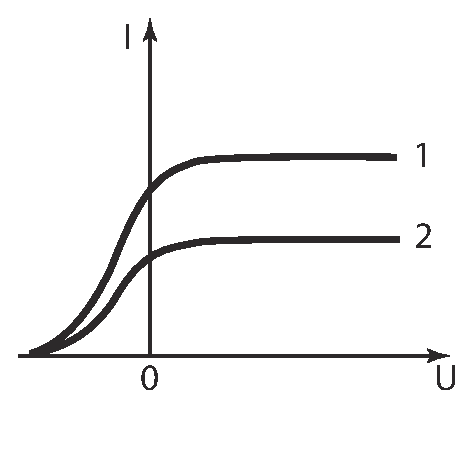
\includegraphics[width=.37\textwidth]{1_12} \hspace*{2em}
        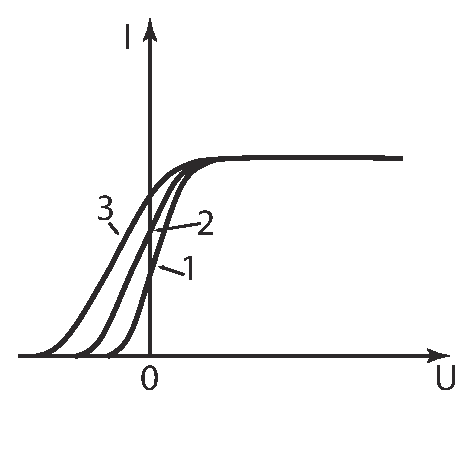
\includegraphics[width=.37\textwidth]{1_13}
        \parbox{.37\textwidth}{\caption{К задаче 1.12} \label{pic1.12}} \hspace*{2em}
        \parbox{.37\textwidth}{\caption{К задаче 1.13} \label{pic1.13}}
    \end{figure}

\item На рисунке \ref{pic1.13} схематически представлены вольт-амперные характеристики
(кривые 1, 2 и 3) фотоэффекта для одного и того же металла. Объясните причину
отличия этих кривых.

\item Проявляются ли волновые свойства фотонов в явлениях фотоэффекта?

\item При эффекте Комптона длина волны смещённой компоненты увеличивается. А
возможно ли обратное (уменьшение длины волны)?

\item Как меняется интенсивность смещённой и несмещённой компонент в эффекте
Комптона при изменении угла рассеяния?

\item Как изменится график зависимости спектральной плотности энергетической
зависимости абсолютно чёрного тела при изменении температуры?

\end{enumerate}